\documentclass [12pt]{article}
\setlength{\parindent}{0em}
\setlength{\parskip}{0.25in}
\usepackage{geometry}
\geometry{verbose,letterpaper,tmargin=0.5in,bmargin=1.0in,lmargin=.70in,rmargin=.70in}
\usepackage{graphicx}
\usepackage{amsmath}
\usepackage{amssymb}
\usepackage{amsthm}
\theoremstyle{definition}
\newtheorem{exmp}{Example}[section]
\usepackage{tikz}
\usetikzlibrary{arrows,decorations.pathmorphing,backgrounds,positioning,fit,petri,calc,matrix}
\usepackage{slashbox}
\usepackage{listings}
\usepackage{ dsfont }
\usepackage{ upgreek }
\usepackage{graphicx}
\graphicspath{ {./images/} }


\definecolor{dkgreen}{rgb}{0,0.6,0}
\definecolor{gray}{rgb}{0.5,0.5,0.5}
\definecolor{mauve}{rgb}{0.58,0,0.82}

\lstset{frame=tb,
  language=Python,
  aboveskip=3mm,
  belowskip=3mm,
  showstringspaces=false,
  columns=flexible,
  basicstyle={\small\ttfamily},
  numbers=none,
  numberstyle=\tiny\color{gray},
  keywordstyle=\color{blue},
  commentstyle=\color{dkgreen},
  stringstyle=\color{mauve},
  breaklines=true,
  breakatwhitespace=true,
  tabsize=3
}

\DeclareMathOperator{\Cspan}{ \CC-span }

\title{Home Work 6}
\author{Madhu Peduri}
\date{03/13/2021}

\begin{document}
\section*{Homework 6}

{\bf 6.5.a.} Let $H = \dfrac{1}{\sqrt{2}}\begin{bmatrix} 1 & 1 \\ 1 & -1 \end{bmatrix}$. Write the matrix of the operator $H[2]$ acting on the space $B^{\otimes 3}$

\phantom{1em} {\bf 1.} We have qubit space of 3 and Hardman operator on subset of 2 qubits, given by below formula,\\
\phantom{1000em} $X[p] = I_{B^{\otimes (p-1)}} \otimes I_{B^{\otimes (n-p)}}$

\phantom{1em} {\bf 2.} In our case $n=3, p=2$, we get, $H[2] = I_{B^{\otimes (1)}} \otimes H \otimes I_{B^{\otimes (1)}}$\\\\
\phantom{1000em} $H[2] = \dfrac{1}{\sqrt{2}}\begin{bmatrix} 1 & 0 \\ 0 & 1 \end{bmatrix} \otimes \begin{bmatrix} 1 & 1 \\ 1 & -1 \end{bmatrix} \otimes \begin{bmatrix} 1 & 0 \\ 0 & 1 \end{bmatrix}$\\\\
\phantom{1000em} $= \dfrac{1}{\sqrt{2}}\begin{bmatrix} 1 & 1 & 0 & 0 \\ 1 & -1 & 0 & 0 \\ 0 & 0 & 1 & 1 \\ 0 & 0 & 1 & -1\end{bmatrix} \otimes \begin{bmatrix} 1 & 0 \\ 0 & 1 \end{bmatrix} = \dfrac{1}{\sqrt{2}}\begin{bmatrix} 1 & 0 & 1 & 0 & 0 & 0 & 0 & 0\\ 0 & 1 & 0 & 1 & 0 & 0 & 0 & 0\\1 & 0 & -1 & 0 & 0 & 0 & 0 & 0\\0 & 1 & 0 & -1 & 0 & 0 & 0 & 0\\0 & 0 & 0 & 0 & 1 & 0 & 1 & 0\\0 & 0 & 0 & 0 & 0 & 1 & 0 & 1\\0 & 0 & 0 & 0 & 1 & 0 & -1 & 0\\0 & 0 & 0 & 0 & 0 & 1 & 0 & -1\end{bmatrix}$

\newpage

{\bf 6.5.b.}\\
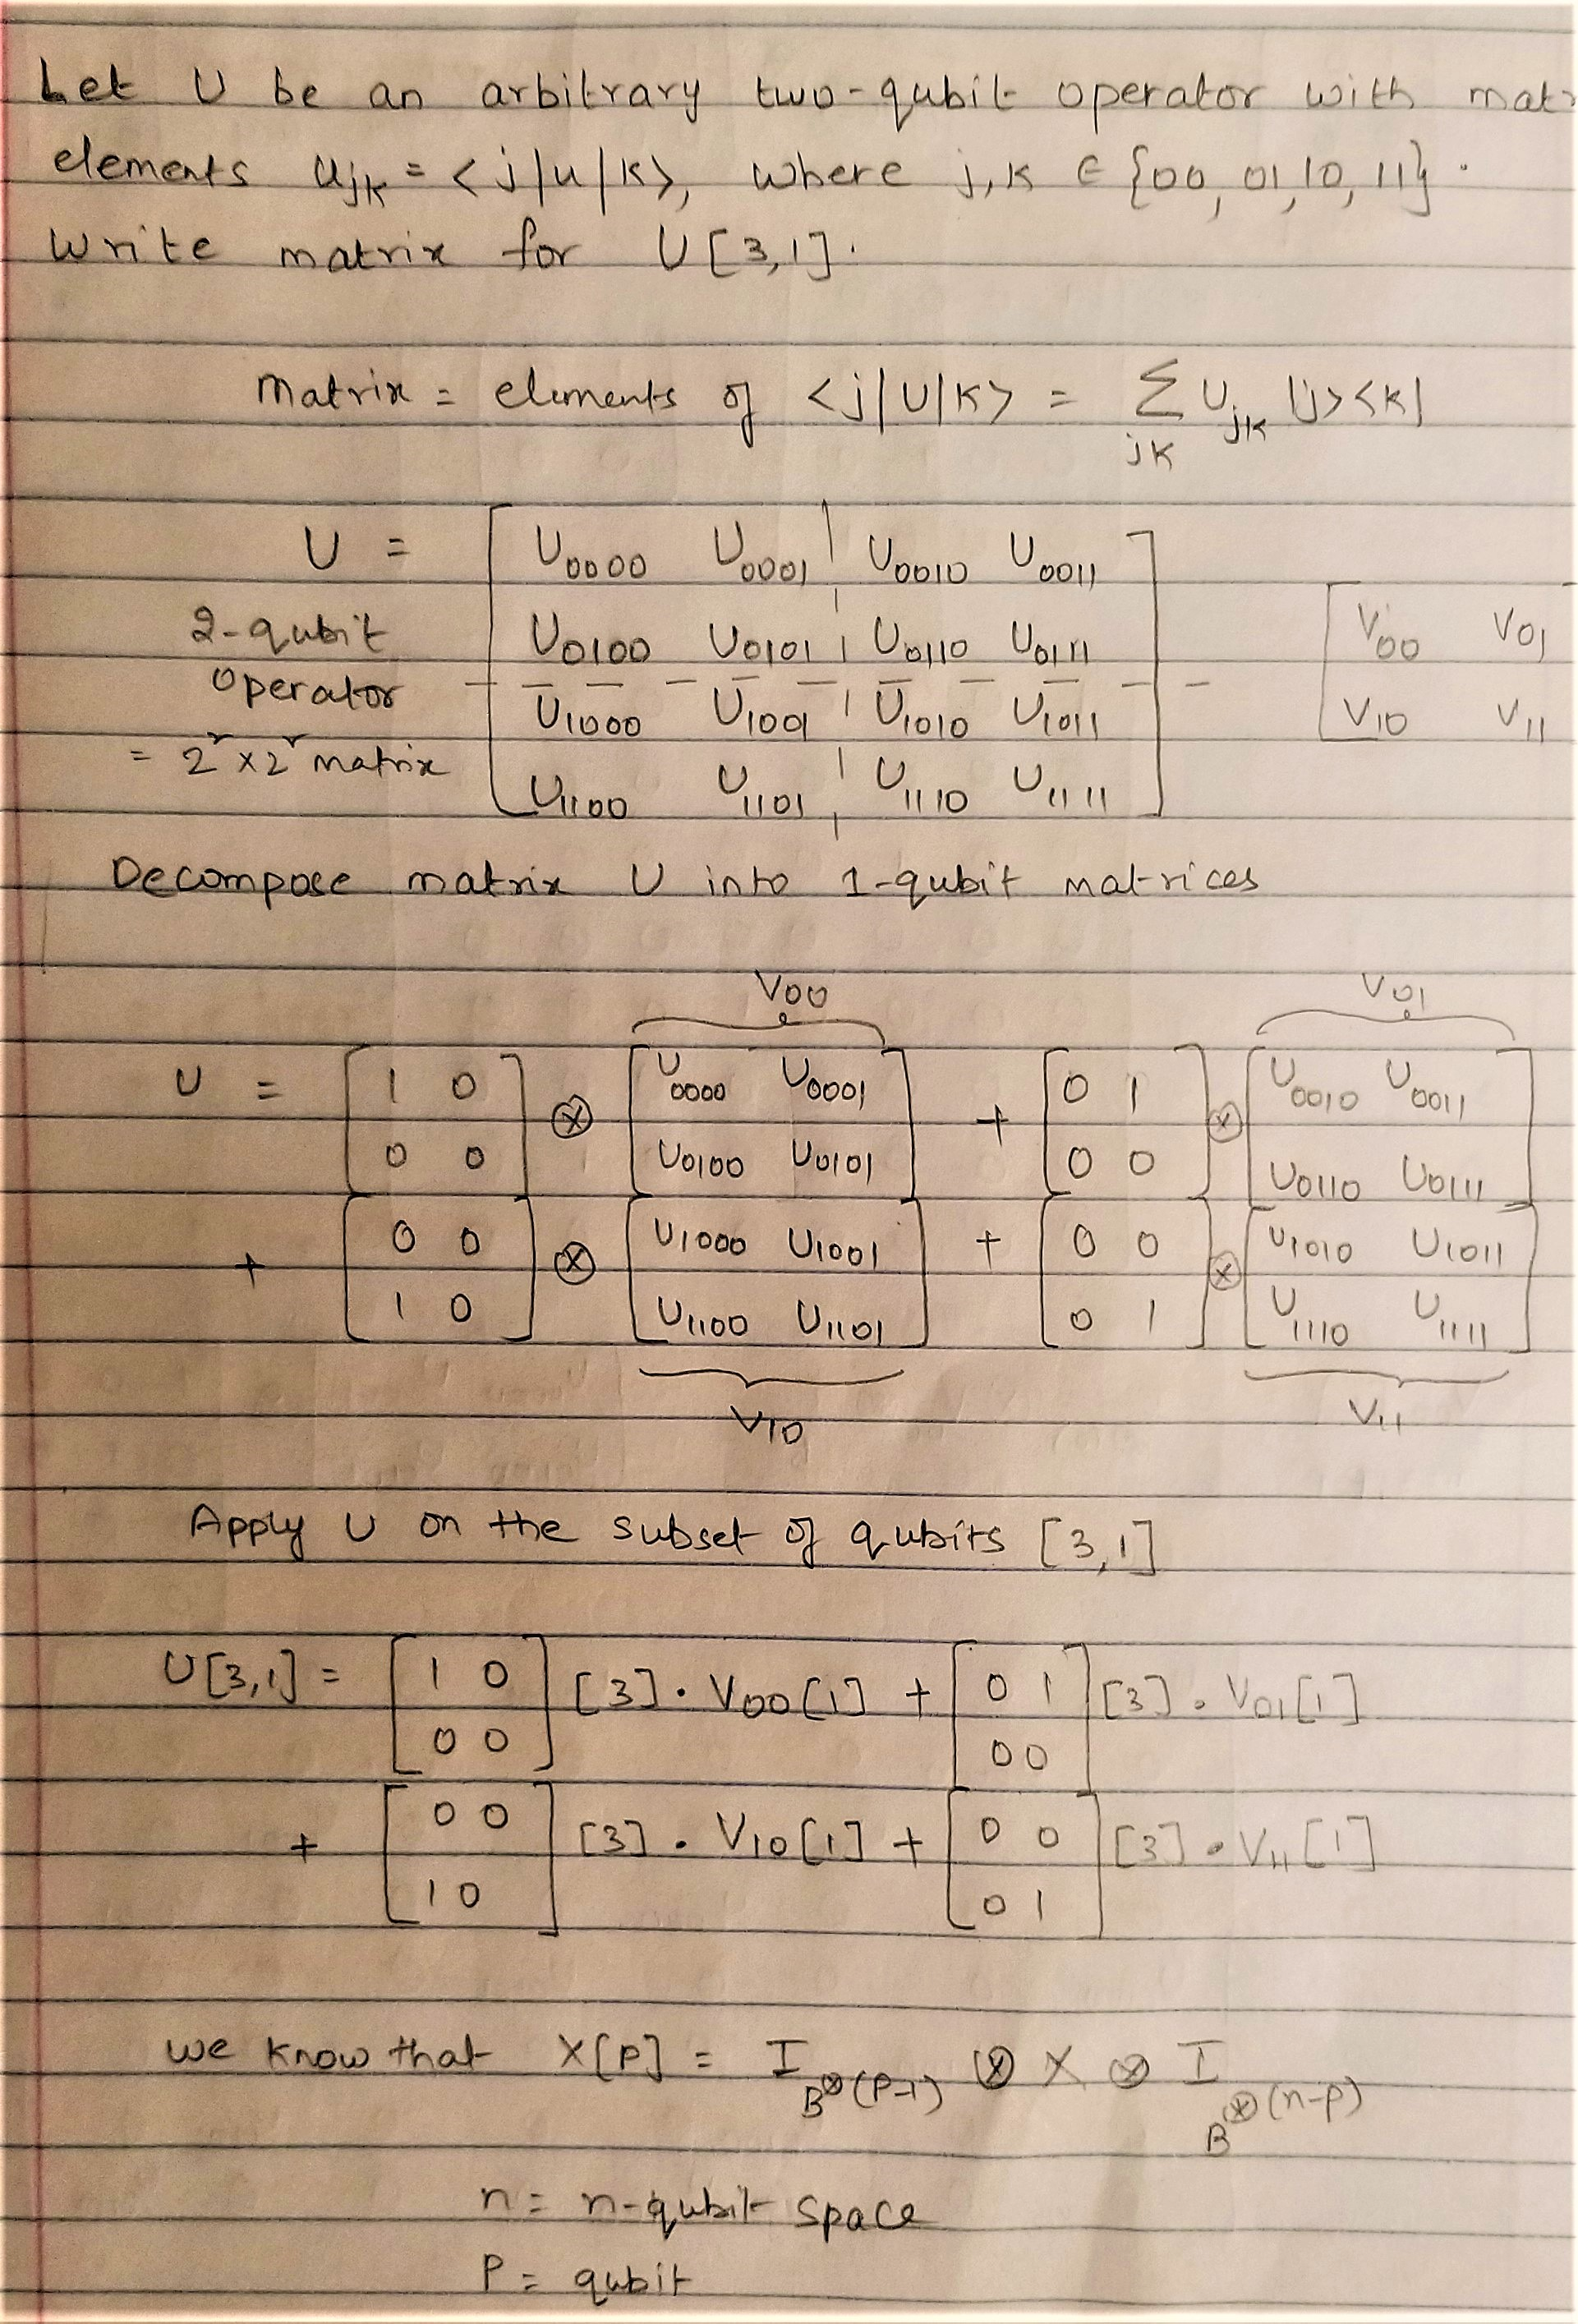
\includegraphics[width=18cm, height=23cm]{I11}\\
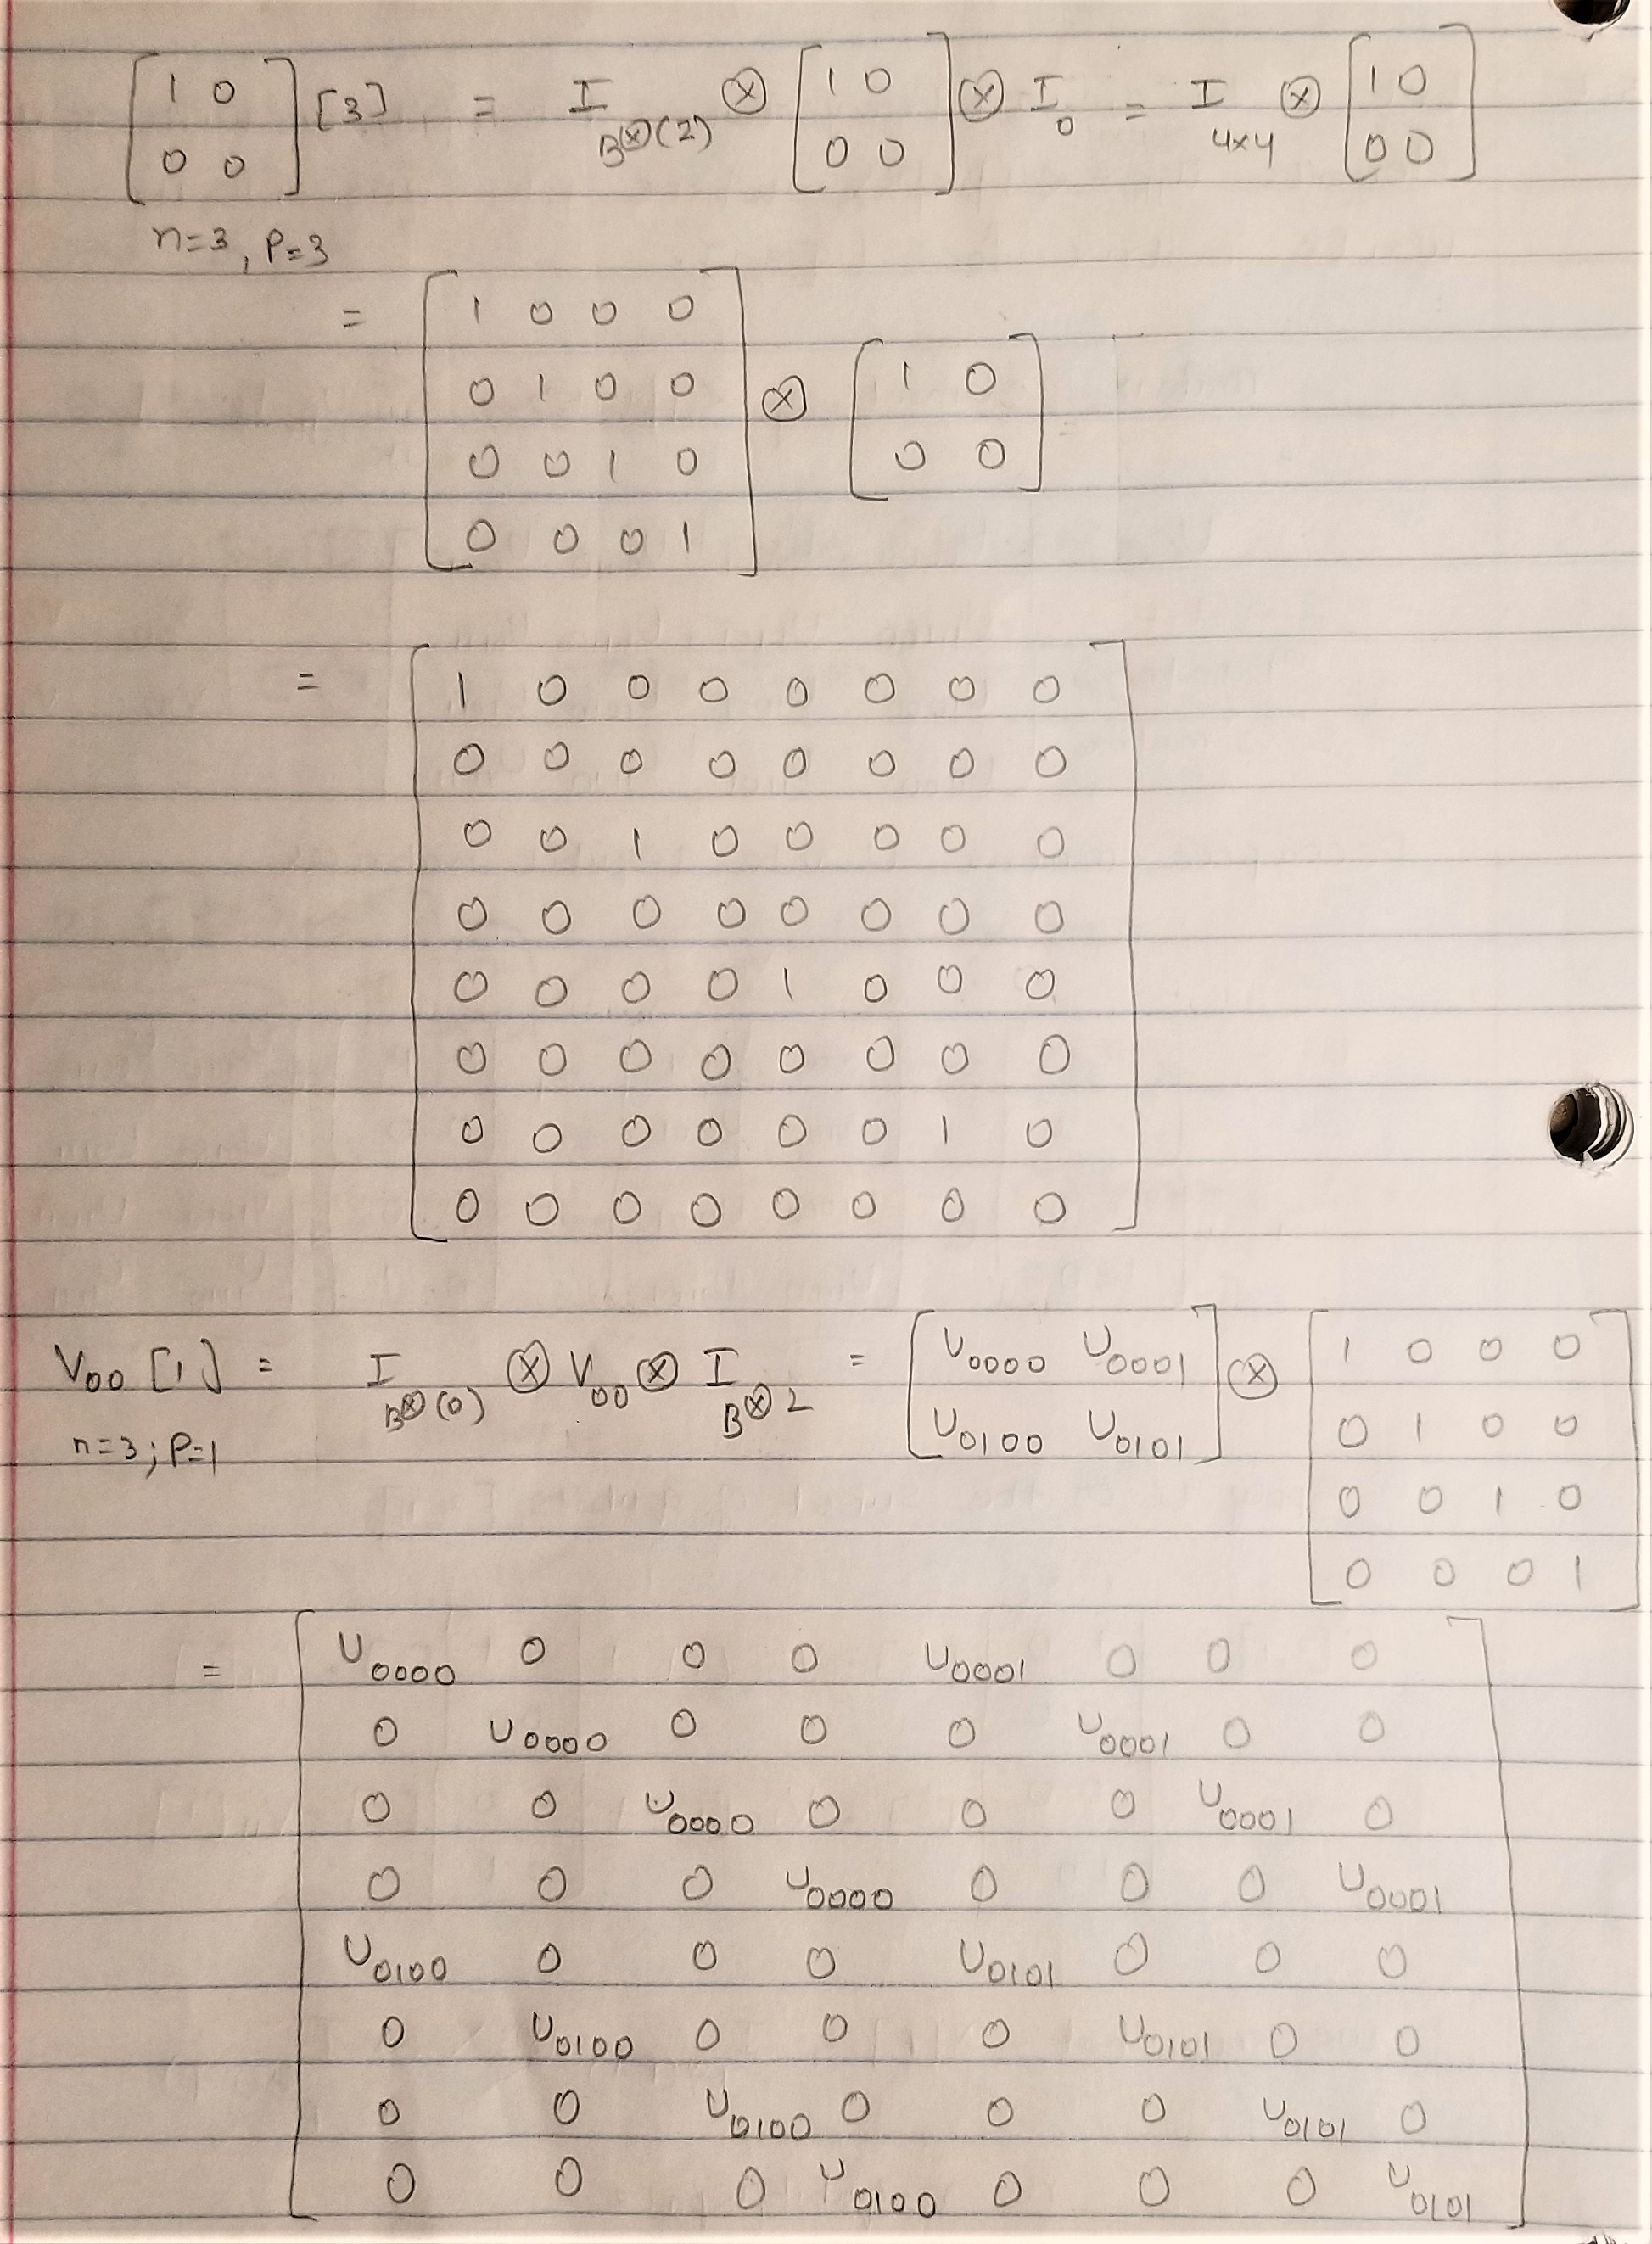
\includegraphics[width=18cm, height=23cm]{I22}\\
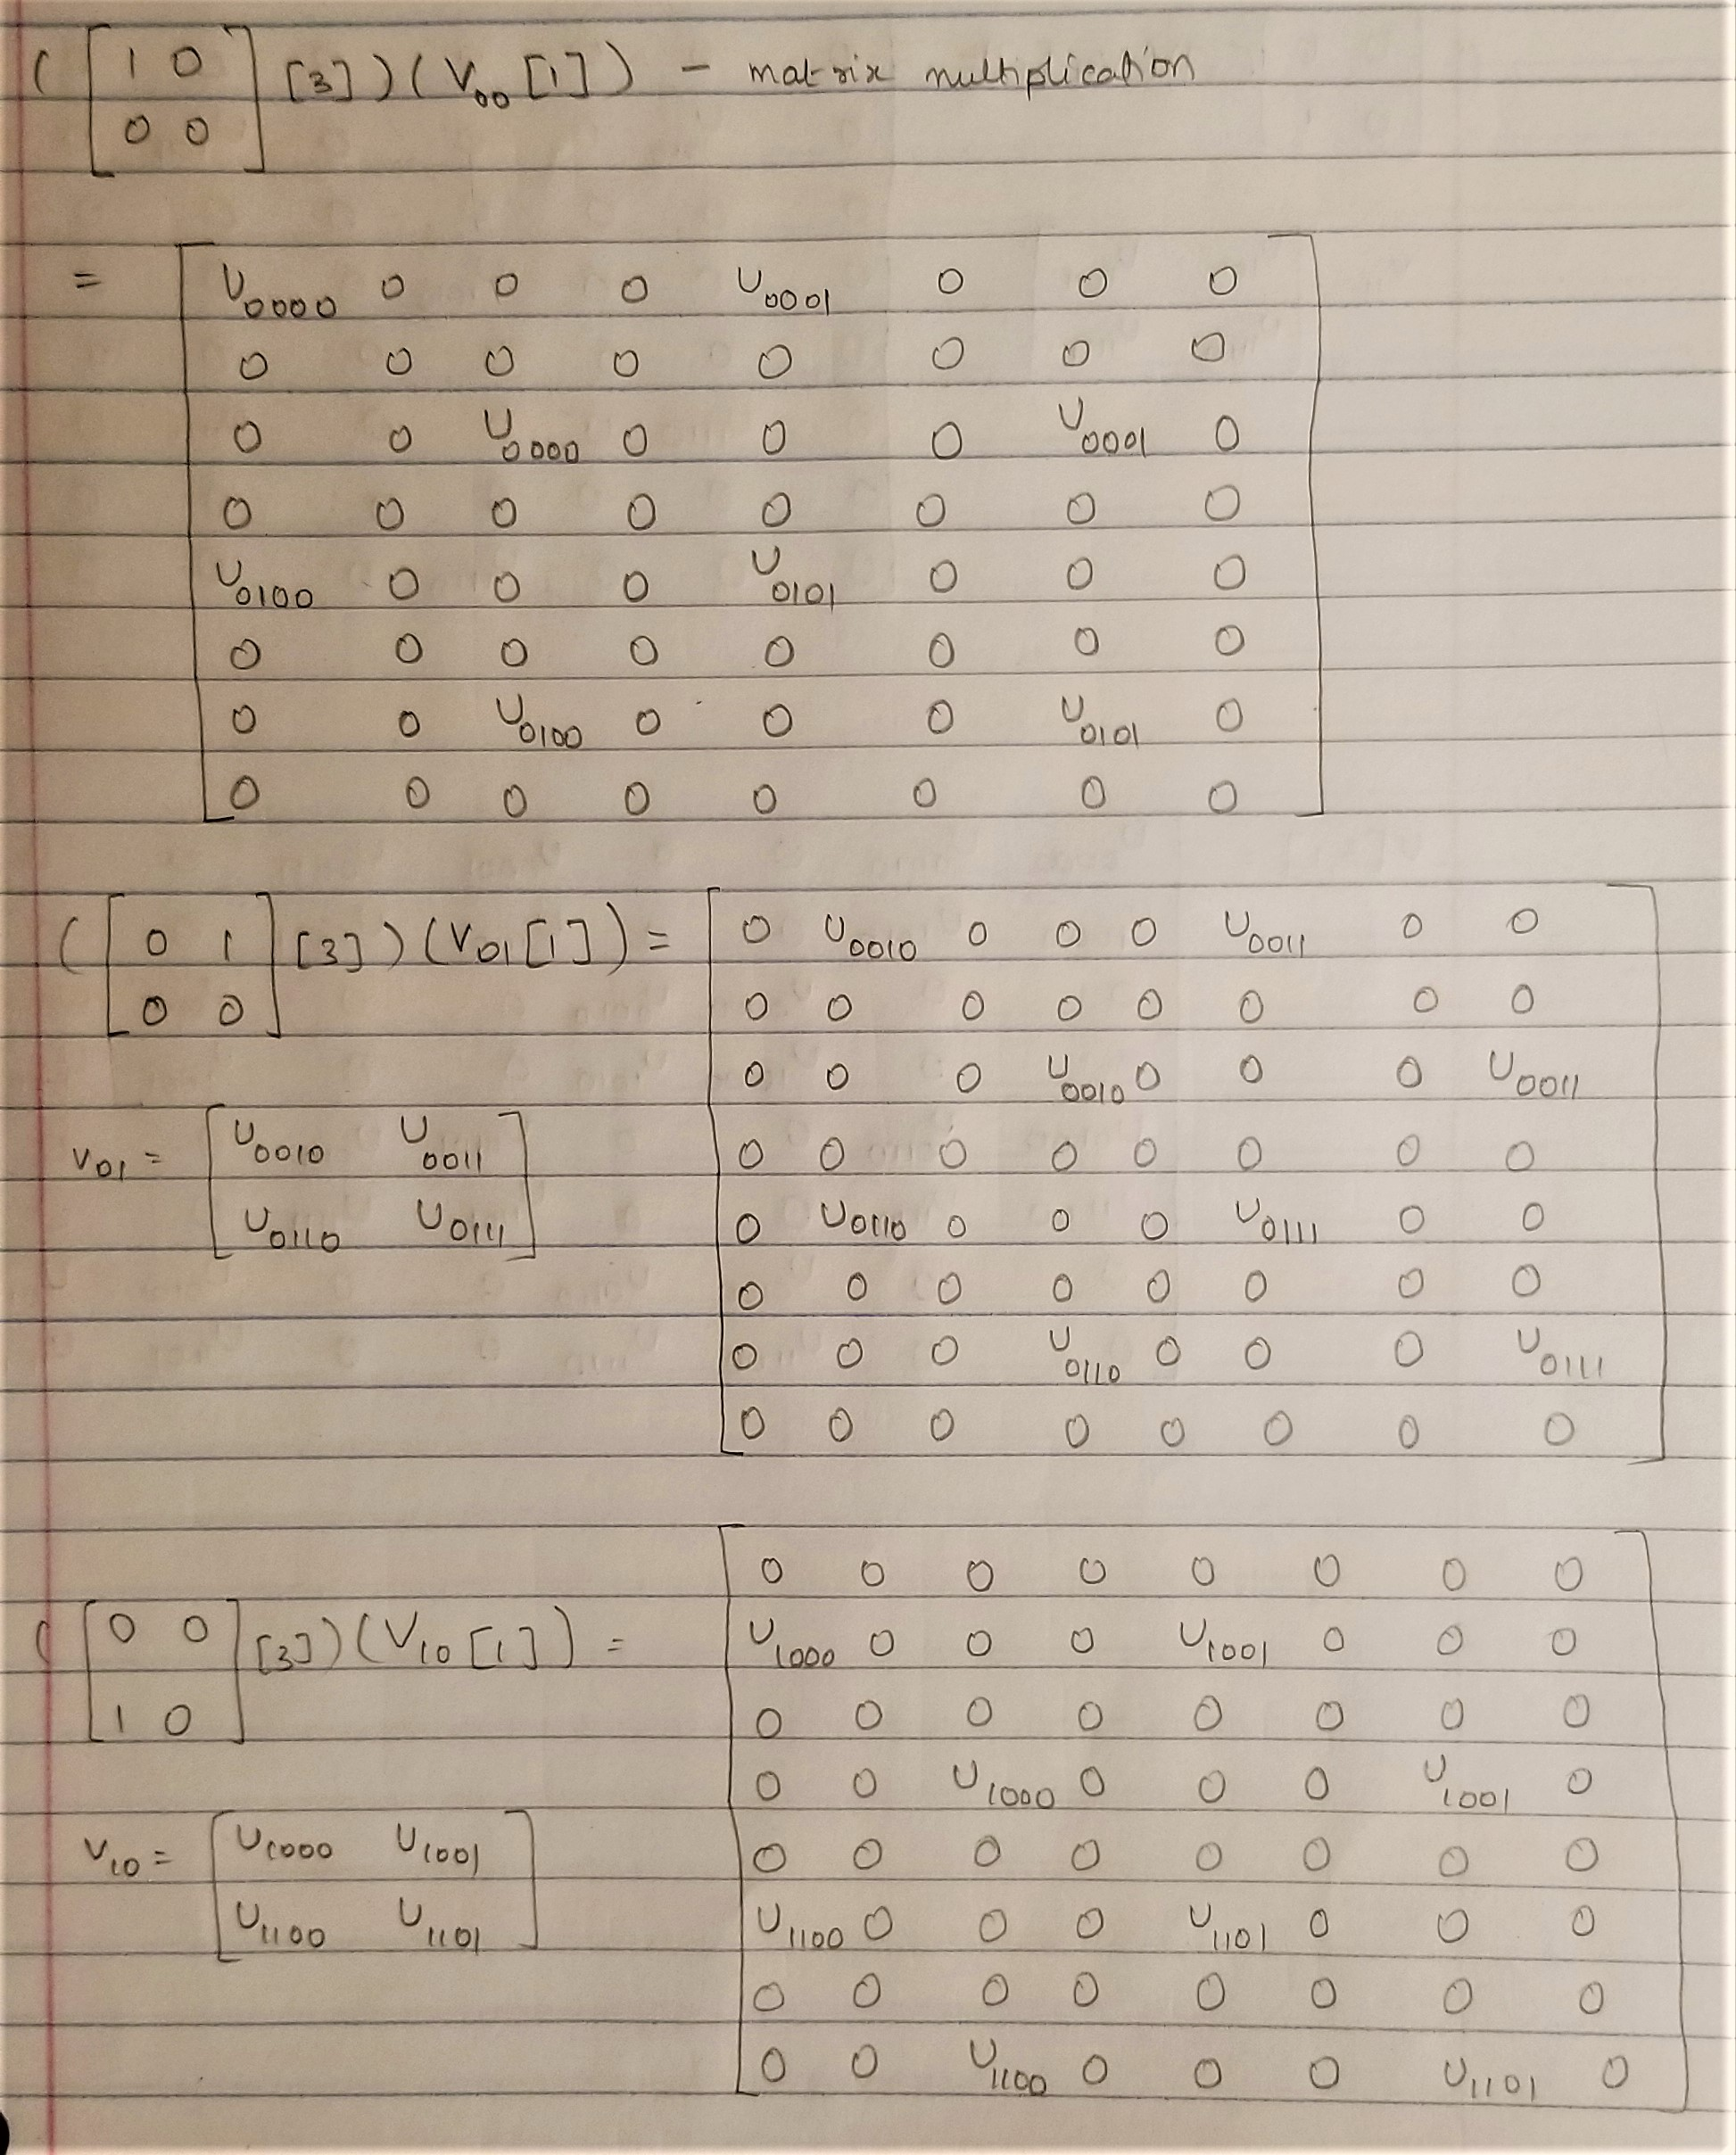
\includegraphics[width=18cm, height=23cm]{I33}\\
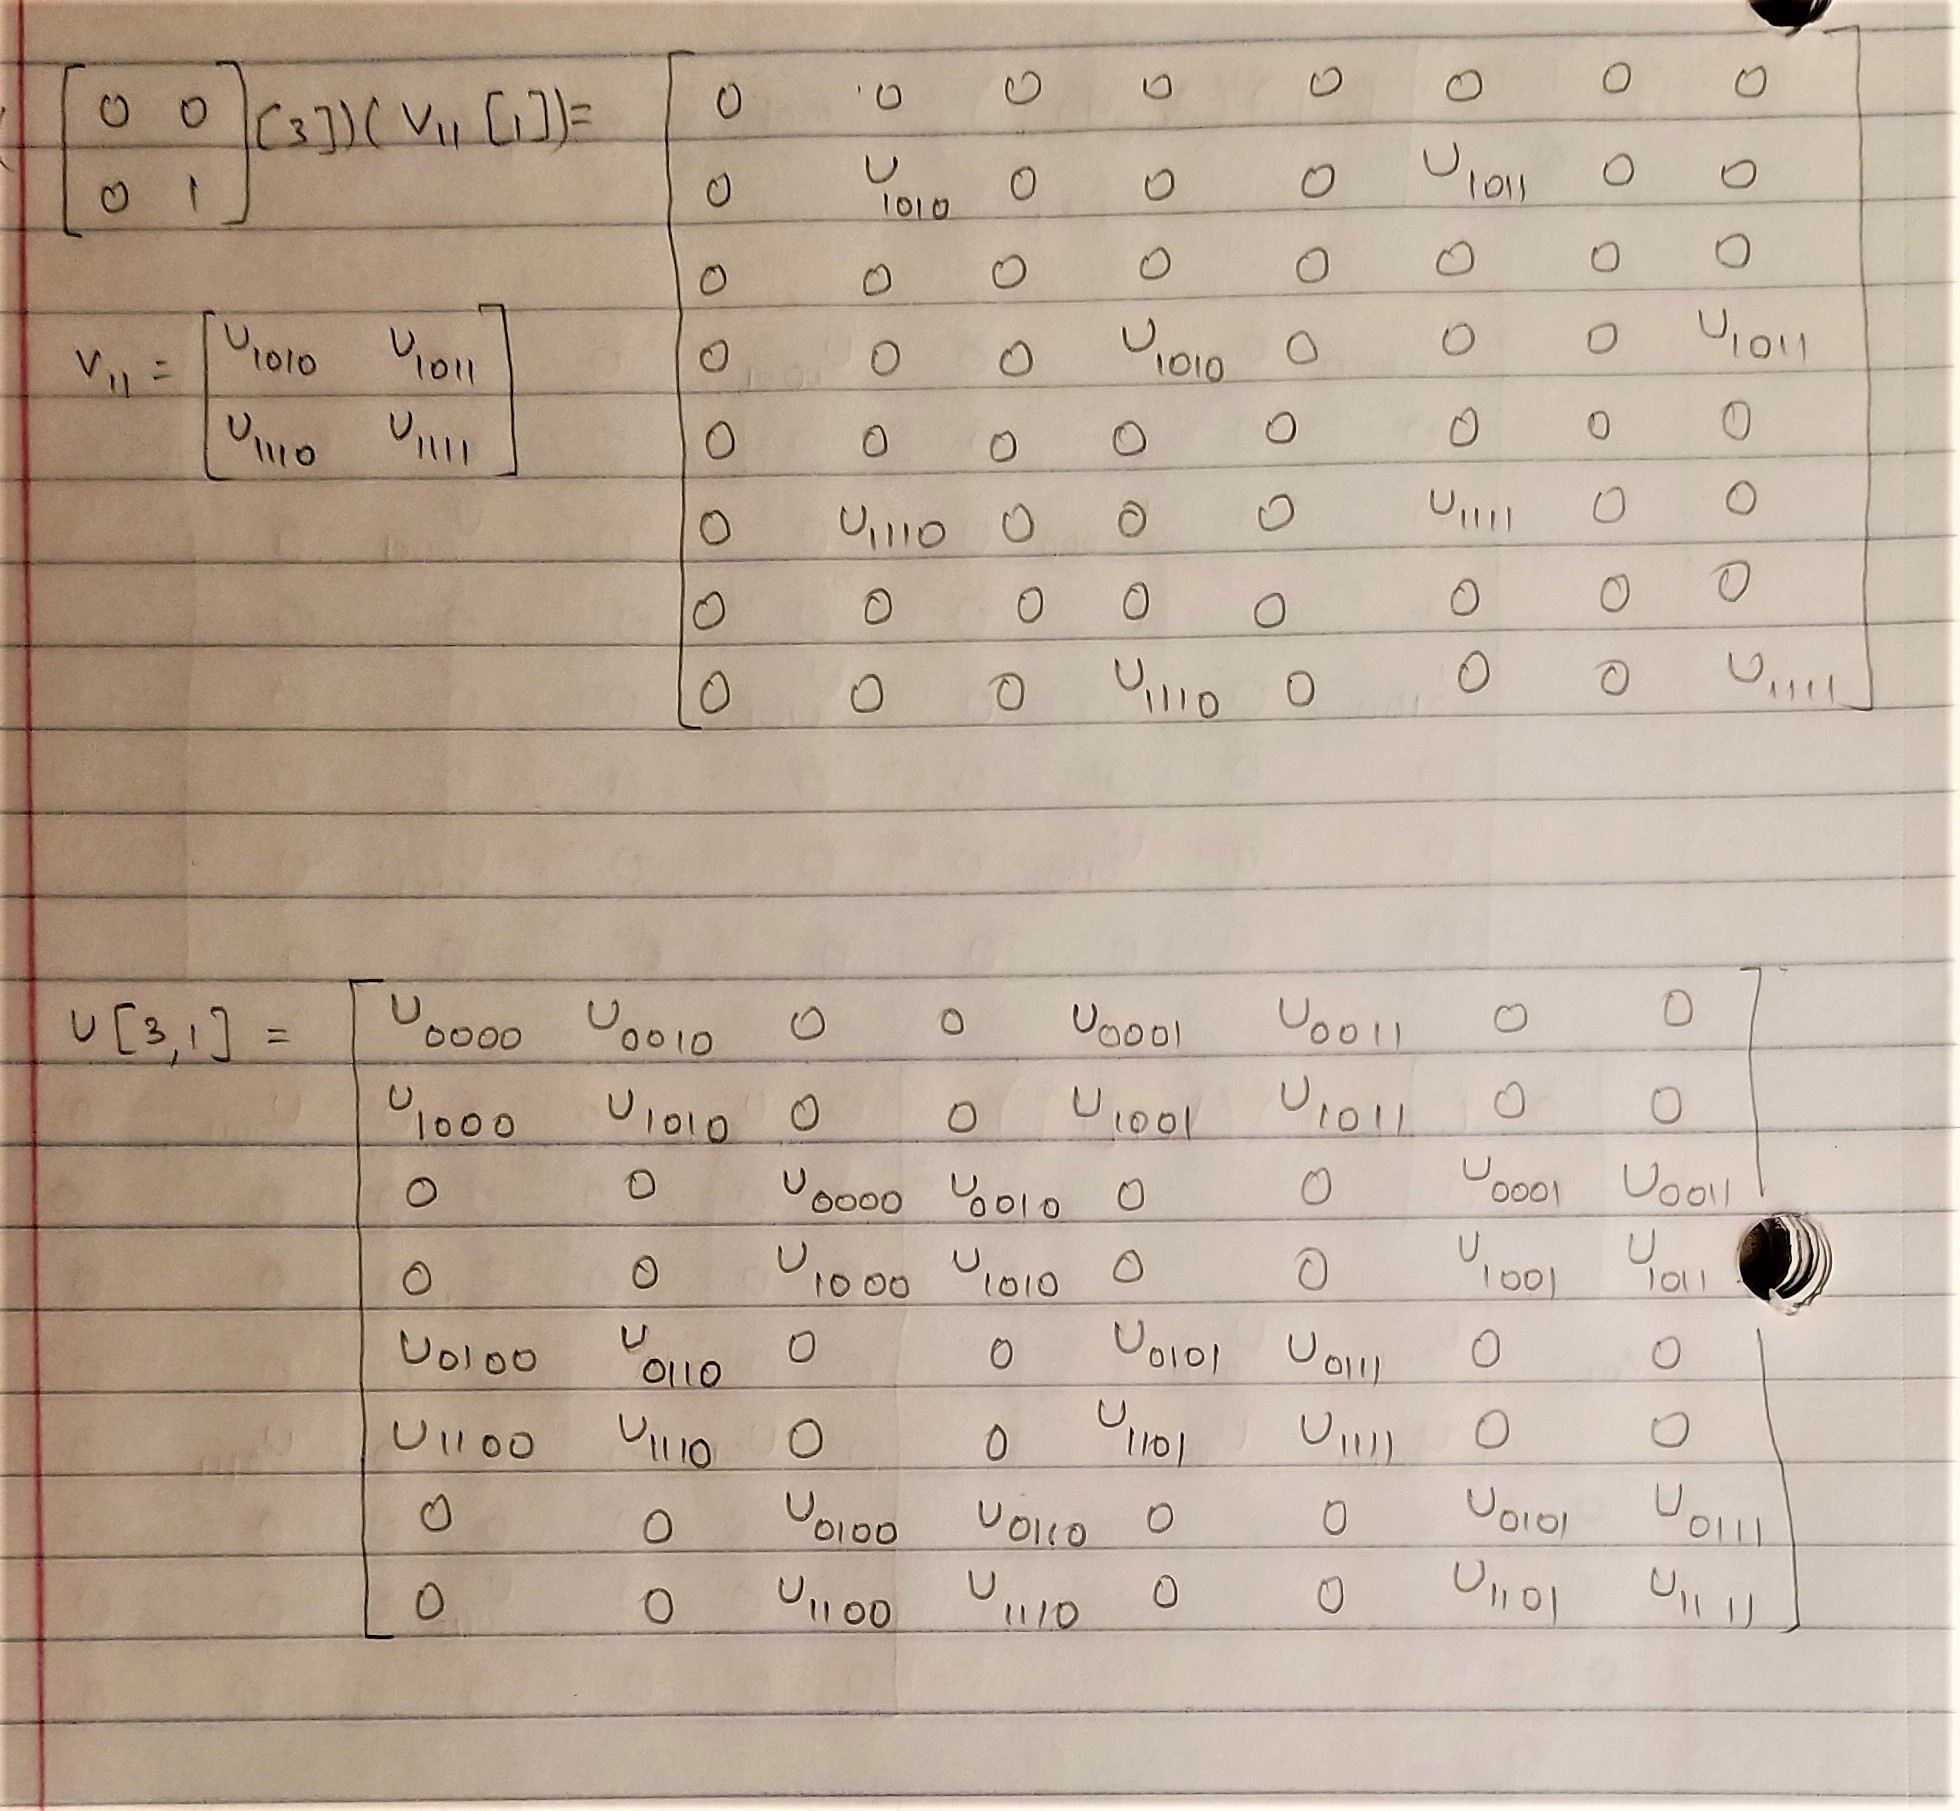
\includegraphics[width=18cm, height=23cm]{I44}

\newpage

{\bf 1.}


\end{document}